% options:
% thesis=B bachelor's thesis
% thesis=M master's thesis
% czech thesis in Czech language
% slovak thesis in Slovak language
% english thesis in English language
% hidelinks remove colour boxes around hyperlinks

\documentclass[thesis=B,czech]{FITthesis}[2012/06/26]

\usepackage[utf8]{inputenc} % LaTeX source encoded as UTF-8

\usepackage{graphicx} %graphics files inclusion
% \usepackage{amsmath} %advanced maths
% \usepackage{amssymb} %additional math symbols

\usepackage{dirtree} %directory tree visualisation

% % list of acronyms


\usepackage[acronym,nonumberlist,toc,numberedsection=autolabel]{glossaries}
\iflanguage{czech}{\renewcommand*{\acronymname}{Seznam pou{\v z}it{\' y}ch zkratek}}{}
\makeglossaries

\usepackage{todonotes}
\usepackage{enumitem}
\usepackage{hyperref}
\usepackage{tabularx}
\usepackage{spverbatim}
\usepackage{listings}
\usepackage{caption}

\DeclareCaptionFont{white}{\color{white}}
\DeclareCaptionFormat{listing}{\colorbox{gray}{\parbox{\textwidth}{#1#2#3}}}
\captionsetup[lstlisting]{format=listing,labelfont=white,textfont=white}

\newcommand{\tg}{\mathop{\mathrm{tg}}} %cesky tangens
\newcommand{\cotg}{\mathop{\mathrm{cotg}}} %cesky cotangens

\newcommand{\GTD}{\textit{GTD }}
\newcommand{\textctandit}[1]{\textit{\uv{#1}}}

% % % % % % % % % % % % % % % % % % % % % % % % % % % % % % 
% ODTUD DAL VSE ZMENTE
% % % % % % % % % % % % % % % % % % % % % % % % % % % % % % 

\department{Katedra softwarového inženýrství}
\title{Systém osobního plánování na základě metodiky Getting Things Done}
\authorGN{Michal} %(křestní) jméno (jména) autora
\authorFN{Sláma} %příjmení autora
\authorWithDegrees{Michal Sláma} %jméno autora včetně současných akademických titulů
\supervisor{Ing. Jiří Mlejnek}
\acknowledgements{Děkuji vedoucímu své práce za hodnotné rady a své rodině za podporu při vytváření této práce.}
\abstractCS{Bakalářská práce obsahuje analýzu osobního plánování na základě metodiky Getting Things Done. Srovnává existující řešení, navrhuje vlastní systém a hledá pro něj vhodné technologie. Součástí práce je implementace aplikaci pro centrální uložení dat vystavující REST API a mobilní aplikaci pro OS Android na principu tenkého klienta. Zároveň navrhuje a obasahuje implementaci publikaci dat na Facebook a Google kalendář. Pro nasazení aplikace instaluje server na portálu DigitalOcean.\todo{pospisuje instalaci}}
\abstractEN{Sem doplňte ekvivalent abstraktu Vaší práce v~angličtině.}
\placeForDeclarationOfAuthenticity{V~Praze}
\declarationOfAuthenticityOption{4} %volba Prohlášení (číslo 1-6)
\keywordsCS{webová aplikace, mobilní aplikace, osobní plánování, spring, android, REST API, Facebook, Google kalendář, DigitalOcean}
\keywordsEN{web application, mobile appliaction, personal planning, spring, android, REST API, Facebook, Google Calendar, DigitalOcean}

\lstset{
	basicstyle=\footnotesize\ttfamily,
	numberstyle=\tiny,
	numbersep=5pt,
	tabsize=2,
	extendedchars=true,
	breaklines=true,
%	showstringspaces=true,
	keywordstyle=\color{red},
	frame=b,         
	stringstyle=\color{white}\ttfamily,
	showspaces=false, 
	showtabs=false,  
	xleftmargin=17pt,
	framexleftmargin=17pt,
	framexrightmargin=5pt,
	framexbottommargin=4pt,
	showstringspaces=false, 
	breakatwhitespace=true,
	commentstyle=\color{pgreen},
	keywordstyle=\color{pblue},
	stringstyle=\color{pred}    
}
\lstloadlanguages{Java}

\begin{document}
 

\newacronym{CVUT}{{\v C}VUT}{{\v C}esk{\' e} vysok{\' e} u{\v c}en{\' i} technick{\' e} v Praze}
\newacronym{FIT}{FIT}{Fakulta informa{\v c}n{\' i}ch technologi{\' i}}
\newacronym{ws}{WS}{Web service}
\newacronym{api}{API}{Application Programming Interface}
\newacronym{os}{OS}{Operating system}
\newacronym{rest}{REST}{Representational State Transfer}
\newacronym{soap}{SOAP}{Simple Object Access protocol}
\newacronym{http}{HTTP}{Hypertext Transfer Protocol}
\newacronym{wsdl}{WSDL}{Web Services Description Language}
\newacronym{crud}{CRUD}{create-read-update-delete operations}
\newacronym{uri}{URI}{Uniform Resource Identifier}
\newacronym{wadl}{WADL}{Uniform Resource Identifier}
\newacronym{raml}{RAML}{RESTful API Modeling}
\newacronym{yaml}{YAML}{Ain’t Markup Language}
\newacronym{xml}{XML}{Extensible Markup Language}
\newacronym{json}{JSON}{JavaScript Object Notation}
\newacronym{orm}{ORM}{Object-relational mapping}
\newacronym{sdk}{SDK}{Software development kit}
\newacronym{sp2}{BIK-SP2}{Software project 2}

\todototoc
\listoftodos

\begin{introduction}
\begin{center}
\textit{\uv{Ze všeho nejvíce požírá čas a energii neustále neproduktivní přemýšlení o věcech, které musíme udělat.}}\\
Kerry Glesson
\end{center}

V současném informačním věku naše práce přestává být fyzickou. Práce už není ohraničena jasnými hranicemi a existuje velké množství informačních zdrojů použitelných pro její zpracování. Řešitel je tím vystaven tlaku nejasného zadání i rozsahu a musí si sám určit cíle své práce.

Naše mysl nejasné nepřijímá, jakékoliv takové úkoly nám neustále připomíná, vyžaduje se jejich řešení a znemožňuje nám tím koncentraci. Potřebujeme nový přístup. Přístup, abychom naši mysl dokázali přesvědčit, že máme vše jasné a právě teď se můžeme koncentrovat pouze na aktuální úkol.

Jedním z takových přístupu je metodika vytvořená Davidem Allenem \GTD\cite{gtd}. Jeho motto \textit{\uv{Jak zvládnout práci i život a cítit se při tom dobře}} je mým kýženým životním cílem.

Moje práce se zabývá rozšířením návrhu a implementace informačního systému pro osobní plánování založeném na metodice GTD, které jsem zpracovával v rámci týmového projektu \acrshort{sp2}. Provedu analýzu samotné metodiky, navrhnu vhodnou infrastrukturu splňující potřebná kritéria \GTD\cite{gtd}, implementuji aplikaci pro centrální uložení dat a mobilní aplikaci pro uživatele.    

	
\end{introduction}

\chapter{Cíl práce}

Cílem práce je analyzovat metodiku \GTD\cite{gtd}, porovnat existující implementace osobního plánování podporující neco. a navrhnout vlastní informační systém.

Navazujicí spojení  dále/pokračuje
Vytvoření aplikaci poskytující \acrshort{ws} pro centrální uložení dat navazující na práci v předmětu \acrshort{sp2}. Vybrat nejvhodnější typ webových služeb. Pro tuto aplikaci najít potřebný hosting a na něm provést konfiguraci aplikačního a databázového serveru.

\todo{napojeni}
Implementace mobilní aplikace pro OS Android využívající \acrshort{ws} služeb centrálního uložení dat a fungující na principu tenkého klienta.   

Prozkoumat postupy pro práci s \acrshort{api} \textit{Facebooku} a \textit{Google kalendáře} s cílem implementovat publikaci úkolu na zeď Facebooku a do Google kalendáře. S tím je spojena integrace přihlášení uživatele pomocí účtů těchto systémů.  

Výsledkem práce nemá být vytvoření odladěné aplikace, ale získání know-how s vývojem takového systému.
  
\chapter{Analýza metodiky \GTD}

V této kapitole se zabývám analýzou metodiky \GTD, hledám její základní stavební prvky a její přínos pro osobní plánování. Definuji důležité pojmy a postupy pro využití v dalším návrhu aplikace. 
Dále srovnávám existující implementace osobního plánování a hledám jejich výhody, kterými podporují kvalitnější a přehlednější osobní plánování.
Na závěr spojuji výsledky obou předchozích bodů a navrhuji základní strukturu a funkce budoucí aplikace.

\section{Metodika GTD - Mít vše hotovo}

Kniha \GTD\cite{gtd} vznikla v roce 2001 a jejím autorem je David Allen. Samotná metodika nepředstavuje jasné řešení, podle kterého se můžeme okamžitě začít řídit a změníme tím svůj život. Snaží se vysvětlit obecné zákonitosti lidské mysli a najít takových způsob plánování, který s ní bude v souladu.\\


Pojďme se na metodiku podívat podrobněji.

\subsection{Změna práce}

Naše práce přestává být fyzikou a přesunuje se do roviny sběru informací, jejich zpracování a vytvoření závěrů. Zároveň nejsme schopni jednoznačně určit prioritu, protože ta se stává proměnnou závislou na mnoha vnějších i vnitřních faktorech. Naše práce přestává mít jasné hranice, které naše mysl potřebuje. Bez jasných hranic nám mysl bude takové věci neustále sama připomínat a požadovat jejich řešení. Paradoxem je, že naše mysl v tomto ohledu nejedná rozumně a připomíná nám naše nedořešené věci bez ohledu na vhodnost situace. Při takovém stavu si říkáme \textit{\uv{nemohu se soustředit}}, mysl nám ruší naši vlastní koncentraci. A koncentrace je nutnou podmínkou pro vysokou výkonnost a my potřebujeme aktuálnímu úkolu věnovat 100\% pozornosti.

Jak toho ale dosáhnout? Potřebujeme naši mysl přesvědčit, že o všech úkolech víme, jsou zaznamenány mimo ní, víme přesně co máme dělat a není riziko zapomenutí.

\subsection{Produktivita}
\begin{center}
\textctandit{Ve znalostní práci není úkol dán, je třeba jej určit. Jaký je očekávaný výsledek práce? Je klíčovou otázkou pro produktivitu znalostních pracovníků. Je to otázka, která si žádá riskantního rozhodnutí. Obvykle na ni neexistuje správná odpověď, místo ní jsou tu možnosti. A má-li být dosaženo produktivity, je třeba jasně specifikovat očekávané výsledky.}\\
Petr Ducken\cite{gtd}
\end{center}

Mysl potřebuje jasný cíl, aby mohla udržet potřebné soustředění, nepřemohla ji únava a dokázala rozlišit důležité informace pro zapamatování.\\
\newline
\textit{Co udělat při zpracování úkolu:}
\begin{enumerate}[nosep]
	\item vyjasnit si požadovaný výsledek
	\item mít jasno o dalším kroku
	\item uložit si úkol do důvěryhodného systému
\end{enumerate}
\vspace*{1\baselineskip}
Začít je třeba od nezákladnější věcí. To nám pomůže zvládnout a odpoutat se od každodenních závazků a poté se můžeme lépe soustředit na větší projekty a vize. Při zpracování potřebujeme využít kontroly ve dvou rovinách: horizontální a vertikální. V horizontální přemýšlíme, co všechno potřebujeme udělat. Ve vertikální řešíme konkrétní věc a co je potřeba vykonat k jejímu splnění.\\ 
\newline
Typický horizontální postup:
\begin{enumerate}[nosep]
\item sběr věcí, které si získaly naší pozornost
\item hodnotíme jejich význam a kroky k jejich splnění
\item uspořádáme si výsledky
\item máme je v plánu a hledáme vhodný čas k provedení
\item provedeme
\end{enumerate}
\vspace*{1\baselineskip}
\subsubsection{Sběr věcí}
Pozornost si získávají věci u kterých si řekneme \textctandit{měl bych}, \textctandit{potřebuji}, \textctandit{musím}. Je potřeba sesbírat všechny věci a žádnou nelze vynechat. Pro naši mysl je důležitým slovem \textctandit{všechno} a nesmí vzniknout jakákoliv pochybnost. V tuto chvíli ještě nepotřebujeme pouze jedno místo uložení, protože spojujeme všechny naše zdroje např. emaily, fyzické dokumenty, \dots Označme taková místa naší schránkou.
\newpage
\subsubsection{Zpracování schránky}

\begin{figure}[h!]\centering
	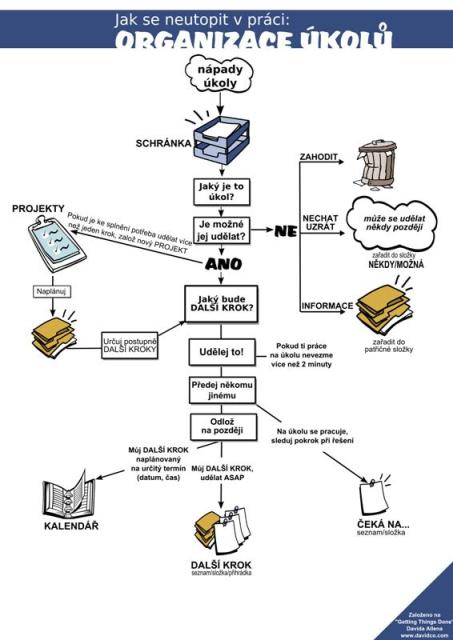
\includegraphics[width=1\textwidth]{pictures/gtd_graph}
	\caption{Digram zpracování schránky dle metodiky \GTD\cite{gtd_graph}}\label{fig:gtd_graph}
\end{figure}

Jak \GTD graf interpretovat (popíši důležité body):
\begin{enumerate}[nosep]
\item Co je to za úkol?
Potřebujeme se nad úkolem zamyslet, čeho se týká a co bude potřeba k jeho splnění. 
\item Realizovatelný/ nerealizovatelný. 
Zde se rozhodujeme, jestli úkol můžeme a chceme splnit. Nerealizovatelný úkol může být pouhá informace. Něco o čem zatím neuvažujeme a nebo pro nás není úkol relevantní a zahazujeme jej.
\item Pro realizovatelné úkoly zjistíme kolik kroků bude potřeba k jejich splnění. V případě, že jich je více zakládáme projekt a pod ním více úkolů. Hierarchie projektů a úkolů má stromovou strukturu, kde úkoly jsou vždy listy stromu.
\item Provedení úkolu
	\begin{enumerate}[nosep]
		\item trvá-li splnění úkolu kratší dobu než 2 minuty - splňme ho
		\item úkol musí vyřešit někdo jiný - deleguj ho
		\item úkol řeším a rozhodnu se o dalším kroku nebo zařadím do kalendáře
	\end{enumerate}
	Po vyhodnocení úkol končí vždy ve stavu, kdy je jasné jeho další zpracování.
\end{enumerate}
\vspace*{1\baselineskip}

Pravidelné vyprazdňování našich schránek představuje práci navíc a z počátku k němu bude existovat odpor. Musíme docílit návyku a plné důvěry, proč to děláme.

Zde už potřebujeme jednotný systém pro správu našich úkolů a projektů. Jeho navržením se budu zabývat v další kapitole.


Důležité pojmy z \GTD
\begin{itemize}
	\item \textit{Činnost/ závazek/ věc/ úkol} -- něco, co máme vykonat a k čemu jsme se zavázali
	\item \textit{Úkol} -- zde ve smyslu konkrétního kroku směřujícího ke splnění činnosti 
	\item \textit{Projekt} -- může obsahovat další \textit{projekty} a úkoly společné pro jednu činnost 
	\item \textit{Schránka} -- místo/ místa na kterých se nacházejí naše činnosti. Zpravidla se jedná o email, šanony,\dots	
\end{itemize}

\subsubsection{Pravidelná kontrola úkolů}

Kritickým klíčem k úspěchu jsou pravidelná zhodnocení všech aktuálních úkolů. Ideálně každý týden. Naším cílem je udržet si plný přehled o úkolem a zohlednit do nich současné priority.

Stejně jako u vyprazdňování schránky se snažíme o vytvoření návyku.

\subsubsection{Co mám dělat?}

Otázkou, kterou si nyní musíme zodpovědět je, jak nám náš seznam úkolů pomůže v rozhodnutí, co nyní dělat.

K tomu nám budou sloužit \textit{kontexty}.

Představme si, že máme chvíli času před schůzkou a po ruce mobilní telefon. Musíme mít možnost rychle zjistit úkoly splnitelné zavoláním z mobilního telefonu. U úkolů zavedeme kontext představující prostředek k jeho splnění. Např. mobilní telefon, notebook, internet, domov,...

Kontexty jsou pro každého z nás specifické a potřebujeme mít možnost si je spravovat.

Dalšími možnými filtry jsou \textit{dostupný čas}, \textit{dostupná energie} (jak moc \uv{svěží} musíme být jeho splnění) a \textit{priorita}.

\subsection{Shrnutí metodiky}

\begin{itemize}
	\item \textit{vše máme mimo naši mysl} --
	cokoliv potřebujeme udělat máme poznamenáno mimo naši hlavu 
	\item \textit{známe další krok}
	\item \textit{umíme naše schránky zpracovat}
	\item \textit{jednotný systém.}
	Máme jednotný systém, kam zaznamenáváme všechny úkoly/ projekty při zpracování schránky. Máme k němu 100\% důvěru a umíme ho správně použít.	
\end{itemize}


\section{Současné implementace}

Zde se seznámíme s existujícími implementacemi pro osobní plánování podporujících metodiku \textit{GTD}. Řešení si vzájemně porovnáme z pohledu ovládání, funkcí z \todo{jak0}pohledu \textit{GTD}, začlenění s emailem, sociálními sítěmi a web, mobilní operační systémy iOS a Android.

\subsection{Toodledo}

Odkaz: www.toodledo.com\cite{gtd_existing_compare_toodledo}\\
Podporovaná zařízení web: ano, iOS: ano, Android: ano

Výhody:
Plně podporuje metodiku GTD. Zakládání a editace úkolů je zde velmi snadná a vše je ukládané okamžitě při změně. U úkolů lze nastavit široké spektrum filtrů od základních kontextů až po definování lokace.
Podporuje Google kalendář (widget).

Nevýhody:
Neobsahuje integraci se sociálními sítěmi.  
Projekty jsou až od placené verze.

Tento systém v současnosti používám pro své osobní plánování.

\begin{figure}\centering
	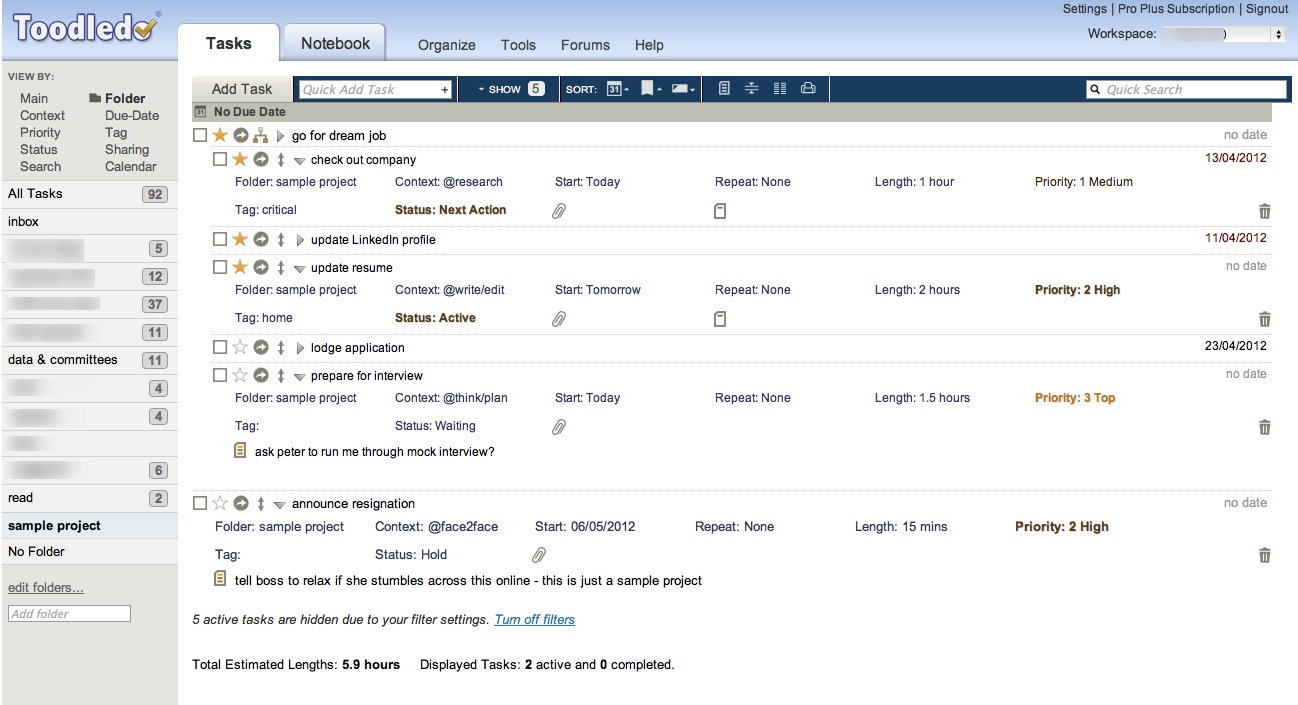
\includegraphics[width=1\textwidth]{pictures/toodledo_overview}
	\caption{Podoba webové aplikace ToodleDo.\cite{toodledo_overview}}\label{fig:toodlefo_overview}
\end{figure}

\newpage

\subsection{Doit.im}

Odkaz: doit.im\cite{gtd_existing_compare_doit}\\
Podporovaná zařízení web: ano, iOS: ano, Android: ano

Výhody:
Plně podporuje metodiku GTD. Příjemná minimalistická aplikace, která je ihned po registraci připravena k použití.  

Nevýhody:
Mírně nepřehledná webová aplikace.

\begin{figure}[h]
	\makebox[\textwidth][c]{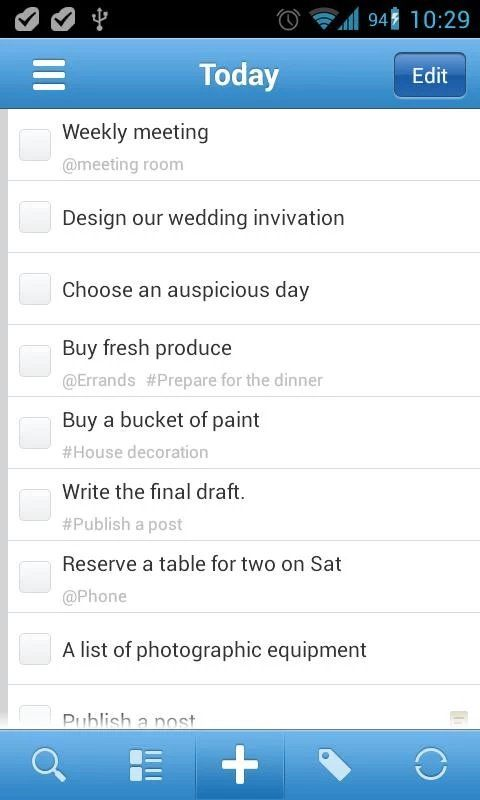
\includegraphics[height=0.7\textwidth]{pictures/doit_overview}}
	\caption{Mobilní aplikace Doit.\cite{doit_overviewgram}}\label{fig:doit_overviewgram}
\end{figure}

\newpage

\subsection{Wunderlist}

Odkaz: www.wunderlist.com\cite{gtd_existing_compare_wunderlist}\\
Podporovaná zařízení web: ano, iOS: ano, Android: ano

Výhody:
Plná podpora \GTD. Pěkné grafické zpracování s další možností přizpůsobení. Po registraci má vše potřebné k okamžitému použití. Jako u ToodleDo jsou změny okamžitě ukládány. Zakládání úkolů zasláním emailu. Sdílení úkolů.

Nevýhody:
Bez sociálních sítí. 

\begin{figure}[h]
	\makebox[\textwidth][c]{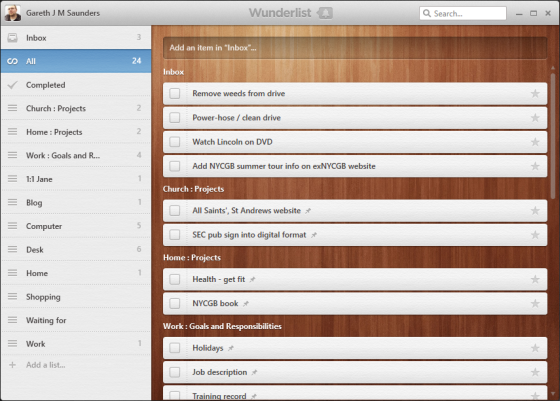
\includegraphics[height=0.7\textwidth]{pictures/wunderlist_overview}}
	\caption{Wunderlist \cite{wunderlist_overview}}\label{fig:wunderlist_overview}
\end{figure}

\newpage
	
\subsection{Todoist}

Odkaz: todoist.com\cite{gtd_existing_compare_todolist}\\
Podporovaná zařízení web: ano, iOS: ano, Android: ano

Výhody:
Projekty jsou zde součástí základní verzí. Pokud chceme jednoduché ovládání bez další funkcí.

Nevýhody:
Nesplňuje nároky \GTD, ale umožňuje všechny potřebné základní funkce. 
Desktopová aplikace vychází z omezení mobilních zařízení a nevyužívá celou šířku obrazovky. 

\newpage
\subsection{Srovnání existujících řešení}

Výsledné srovnání je shrnuto v tabulce \ref{tab:gtd_existing_compare}.

\begin{table}[h!]\centering
	\caption{Porovnání existujících implementací metodiky \textit{GTD} - (* značí placenou verzi)}\label{tab:gtd_existing_compare}
	\begin{tabular}{|m{3cm}|m{2cm}|m{2cm}|m{2cm}|m{2cm}|}\hline
		Funkce& ToodleDo		& Doit.im & Wunderlist & ToDoList \tabularnewline \hline \hline
		Web/Android/iOS& ano/ano/ano& ano/ano/ano& ano/ano/ano& ano/ano/ano\tabularnewline \hline				
		Automatické ukládání& ano& ne& ano& ne\tabularnewline \hline
		Intuitivní ovládání& ano& mírně nepřehledné& ano& ano\tabularnewline \hline		
		Podpora Google kalendáře& ano*& ano & ano& ne\tabularnewline \hline	
		Facebook& ano*& ne& ne& ne\tabularnewline \hline				
	\end{tabular}
\end{table}

\section{Shrnutí analýzy metodiky \GTD}

Z samotné metodiky \GTD jsem odvodil tyto nároky na aplikaci:
\begin{itemize}
\item \textit{Základní funkce.}
Není třeba vytvářet složité funkce. Ale ty které existující, musí být spolehlivé a uživatel nesmí mít problém s jejich ovládáním. 
\item \textit{Dostupnost.}
Aplikace se nemůže soustředit pouze na jednu platformu a musí být dostupná z více platforem (web, mobilní zařízení,...). 
\item \textit{Spolupráce s aplikacemi třetích stran.}
U uživatele lze očekávat Facebook/ Gmail účet a aplikace může toho využít.
\end{itemize}

Současné implementace můj závěr potvrzují. I u malých projektů je podpora pro všechny platformy téměř samozřejmostí. Minimalistické na funkčnost zaměřené uživatelské rozhraní. Synchronizace k emailovými účty je často také přítomna, ačkoliv je už součásti placené verze.

\textit{Implementace bude obsahovat}
\begin{itemize}
\item \textit{Aplikace pro centrální uložení dat vystavující \acrshort{ws} pro jejich správu}
\item \textit{Aplikace pro OS Android}
\end{itemize}

\chapter{Návrh}

Tato kapitola popisuje volbu technologií pro implementovanou aplikaci poskytující centrální uložení dat skrze \acrshort{ws} a aplikaci pro \acrshort{os} Android. Nároky na technologie vycházejí ze závěrů analýzy předešlé kapitoly a dále je rozvíjejí.
Protože jedna z aplikací potřebuje hosting, budeme hledat vhodný server splňující naše potřeby.

Seznámíme se postupem pro propojení mobilní aplikace na Facebook a Google kalendář. Přidělíme každé aplikaci oddělené úkoly. Mobilní aplikace zajistí přihlášení uživatele a získání access tokenu. Tento token předáme aplikaci pro centrální uložení dat a ta zajistí samotnou práci s API protistrany.

Dále kapitola specifikuje REST API a ukazuje webového vývojového prostředí od společnosti Mulesoft, které je k návrhu použito. 

Kapitola dále popisuje vytváření datového modelu.

\section{Rozdělení aplikace}

Ze závěrů analýzy vzešlo, že aplikace musí být pro uživatele dostupná více platformách zahrnující např. mobilní zařízení a web. Proto jsem se rozhodl rozdělit návrh aplikace na dvě části. První bude zajišťovat centrální uložení dat. Druhá pak zajistí pro uživatele samotné GUI pro osobní plánování a správu dat deleguje na první aplikaci. Díky tomuto návrhu se zbavím nutnosti implementovat uložení dat na každé uživatelské aplikaci.

\subsection{Aplikace pro centrální uložení dat}

Skrze \acrshort{ws} bude poskytovat centrální uložení dat do databáze. Služby budou dostupné přes internet a samotná aplikace bude nasazena na aplikační server. Současně umožní publikovat na Facebook a Google kalendář. 

\subsection{Mobilní aplikace pro Android}

První implementace GUI cílená na mobilní zařízení se systémem Android. Fungovat bude na  principu tenkého klienta\cite{gtd_thin_client}. Aplikace využije přihlašovací komponenty Facebooku a Googlu pomocí kterých získá uživatel prostředek pro autorizaci aplikace a přístup k publikaci dat do těchto sítí.

\subsection{Model nasazení}

\begin{figure}[h!]\centering
	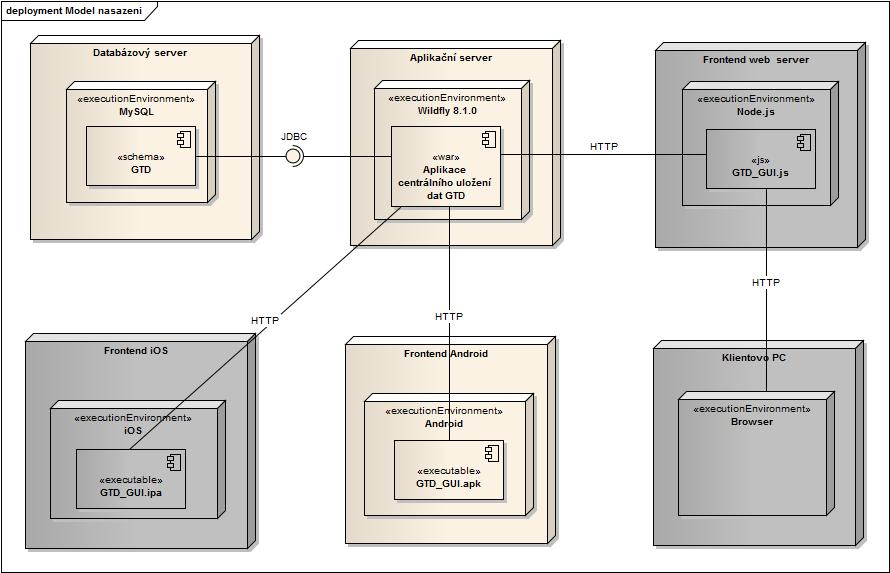
\includegraphics[width=1\textwidth]{pictures/gtd_deployment_model}
	\caption{Model nasazení GTD (šedivě jsou zbarvena úvaha dalšího rozšíření)}\label{fig:gtd_deployment_model}
\end{figure}

Vycházení z návrhu rozdělení aplikace. GUI aplikace jsou unikátní pro každou platformu s centrální aplikací pro správu dat komunikují přes HTTP protokol. Část nasazení \textit{Frontend web server} zobrazuje aplikaci vytvořenou v rámci týmového projektu \acrshort{sp2}. Ta není v současnosti funkční a není součástí nasazení. 

\section{Facebook a Google kalendář}

Aplikace pro osobní plánování nesmí být izolovanou. Zde si rozebereme návrh pro integraci do Facebooku a Google kalendáře. 

\subsection{Facebook}

\subsubsection{Proč Facebook}
Facebook\cite{design_facebook} je v současnosti dominantní sociální sítí a jeho používání se pro mnohé stává denní samozřejmostí\cite{design_facebook_usage}. Poskytuje širokou možnost integrace např. \cite{design_facebook_integration}.

Vývoj na \textit{zdi} uživatele se pro většinu jedinců stává moderním elektronickým deníkem. Do něj chtějí zaznamenávat co nejvíce svých osobních a sociálních informací.

\subsubsection{Oddělení přihlášení od publikace}
\label{design:facebook_divide_appliaction}
	
K oddělení funkce nastane pro přihlášení uživatele a publikace.
Android aplikace umožní uživateli přihlášení k Facebooku s cílem získat access token. Tento token bude následně předán aplikaci pro centrální uložení dat současně s informací identifikující úkol. Ta zajistí jeho publikaci.

Více k access tokenu na \cite{design_facebook_access_tokens}.

\subsubsection{Přihlášení}

Bude zajišťováno na straně Android aplikace.
\newline

\todo{vice rozebrat, propojit, okecat}

Musíme řešit:
\begin{itemize}[nosep]
	\item \textit{registrace aplikace na straně Facebooku}
	\item \textit{nastavení naší aplikace}
\end{itemize}
\vspace*{1\baselineskip}

\textit{Registrace aplikace na straně Facebooku}

Provádí se přes stránky \href{''https://developers.facebook.com/''}{Facebook developer}\cite{design_facebook_developer}. Příklad postupu lze najít na \cite{design_facebook_registration_example}. 
\newline

\textit{Nastavení aplikace}

Pro přihlášení uživatele využijeme komponentu a funkce z SDK Facebooku pro Android viz. \ref{technology:facebook_sdk}. Pro další nastavení budeme postupovat podle návodu v \cite{design_facebook_android_login}.

Komponenta zajistí správu nad procesem přihlašování uživatele. Výstupem procesu přihlášení je objekt obsahující access token.

\subsubsection{Publikace}

Access token umožní autorizaci vůči Facebook API v rámci uživatelem schválených práv. V našem případě budeme mít přístup k editaci zdi uživatele.

Testy nad Facebook API lze skrze \ref{design_facebook_grapapi_explorer}.

%******************** GOOGLE ***********************

\todo{vice oddelit od facebook kapitoly - jine nadpisy/ form8tovani zmenineni podobnosti}
\subsection{Google kalendář}

\subsubsection{Proč Google kalendář}

Google kalendář je součástí rodiny Google aplikací\cite{design_google_apps}. Ze statistik pro Gmail\cite{design_google_usage} můžeme odvodit, že se jedná o rozšířenou součást osobního i firemního plánování.

Google kalendář dále umožňuje synchronizaci do dalších aplikací (např. \href{''https://tools.google.com/dlpage/gappssync''}{MS Outlook}\footnote{tools.google.com/dlpage/gappssync}) a pro odlišné platformy existují další aplikace zobrazení jeho dat (např. \href{''https://play.google.com/store/apps/details?id=org.withouthat.acalendar&hl=cs''}{aCalendar}\footnote{play.google.com/store/apps/details?id=org.withouthat.acalendar} pro Android). 

\subsubsection{Oddělení přihlášení od publikace}

Stejně jako u Facebooku \ref{design:facebook_divide_appliaction} oddělíme funkci na přihlášení a publikaci.

Více o access tokenu na \cite{design_google_access_token_guilde}.

\subsubsection{Přihlášení}

Bude zajišťováno na straně Android aplikace.
\newline

Musíme řešit:
\begin{itemize}[nosep]
	\item \textit{registrace aplikace na straně Google}
	\item \textit{nastavení naší aplikace}
\end{itemize}

\vspace*{1\baselineskip}
\textit{Registrace aplikace na straně Google}

Provádí se přes stránky \href{''https://console.developers.google.com''}{Google developer console}\cite{design_google_console}. Příklad postupu lze najít na \cite{design_google_registration}. 
\newline

\textit{Nastavení aplikace}

Pro přihlášení uživatele využijeme komponentu a funkce z Google play service viz. \ref{technology:google_play_service}. Komponentou bude Google+ Sign-in \cite{design_google_signin_googleplus}. Pro další nastavení budeme postupovat podle návodu v \cite{design_facebook_android_login}.\newline

Samotný proces přihlášení bude mít dvě fáze. V první kroku vyzveme uživatele k přihlášení pomocí svého google účtu. Po tomto kroku ještě nemáme nutný přístup a musí následovat další krok, ve kterém uživatele požádáme o přidělení práv pro naši aplikaci. Tím získáme potřebný access token\cite{design_google_access_token}. 

\subsubsection{Publikace}

Access token umožní autorizaci vůči Google API v rámci uživatelem schválených práv. V našem případě budeme mít přístup k datům v jeho Google kalendáři s právem editace a vyváření.

Testy nad Google API lze skrze \cite{design_google_playground}.

%******************** /GOOGLE ***********************
 
\section{Technologie}

V této části si představíme technologie potřebné pro následující implementaci.

\subsection{Aplikace pro centrální uložení dat}
  
\subsubsection{Webová služba -- \acrshort{rest} \acrshort{api}}

Při volbě webového \acrshort{api} jsem se rozhodoval mezi dvěma typy webových služeb.
\newline
\begin{itemize}[nosep]
	\item \textit{SOAP}
	\item \textit{REST}
\end{itemize}
\vspace*{1\baselineskip}

\todo{pridat sloupec s odkazy na literaturu / odkazy omezit nebo neco jineho}
Nyní se soustředím na hlavní rozdíly mezi těmito službami.
\newline
\begin{table}[h!]\centering
\caption{Rozdíly mezi SOAP a REST}\label{tab:ws_compare}
\begin{tabular}{|p{3cm}|p{3cm}|p{5.5cm}|}\hline
Typ		& SOAP		& REST \tabularnewline \hline \hline
Formát dat\cite{ws_compare_swati}		& XML		& nezávislý (XML, JSON, plain) \tabularnewline \hline
Protokol\cite{ws_compare_swati}		& více možných (HTTP, SMTP,..)		& HTTP \tabularnewline \hline
Možnost cachování\cite{ws_compare_swati}		& ne		& ano \tabularnewline \hline	
Formát specifikace\cite{ws_compare_table}\cite{ws_compare_soapui} & WSDL\cite{ws_soap_wsdl}	& existují formáty jako \acrshort{wadl}\cite{ws_wadl}, Swagger\cite{ws_swagger}, \acrshort{raml}\cite{ws_raml} a další, ale žádný nemůžeme považovat na hlavní \cite{ws_comparison} \tabularnewline \hline 		 
Vystavuje\cite{ws_compare_steve}		& operace & zdroje \tabularnewline \hline
Zabezpečení\cite{ws_compare_steve}		& SSL + WS-Security & SSL \tabularnewline \hline  
Rozšířenost\cite{ws_compare_steve}		& \multicolumn{2}{p{8.5cm}|}{REST získává na stále větší popularitě . Příkladem uvedu např. Google, který se nahradil své dřívější SOAP API právě RESTem.}  \tabularnewline \hline 
Rychlost zpracování\cite{ws_compare_armel} 	& \multicolumn{2}{p{8.5cm}|}{XML parsing je pomalejší než JSON\cite{ws_compare_xml_json_process}}  \tabularnewline \hline 	 		  		
Jednodušší implementace\cite{ws_compare_swati}		&\multicolumn{2}{p{8.5cm}|}{u RESTu na straně klienta i serveru} \tabularnewline \hline 	 				
\end{tabular}
\end{table}

\todo{pouzivam zabezpeceni}
Návrh nepočítá s využitím zabezpečení (přihlášení bude řešeno pomocí tokenu \ref{realization:user_autentorization})  a komunikace bude probíhat přes HTTP protokol (SOAP ztrácí výhodu).
Myšlenkou RESTu je poskytnout CRUD\cite{ws_compare_steve} operace nad vystavenými zdroji\cite{ws_crud} a to přesně odpovídá potřebám navrhovaného centrálního uložení dat.  Mezi další výhody patří rychlá implementace a přenos dat ve formátu JSON.

\todo{vice zduvodnit}
Volba pro \acrshort{ws} je REST.\newline

\label{ws_compare_mulesoft}
Pro specifikaci REST API bude použit jazyk \acrshort{raml}. Jedná se nový jazyk založený na formátu \acrshort{yaml}, který v říjnu 2014 přešel do verze 1.0\cite{ws_raml} a na jehož vývoji se podílí technologičtí odborníci ze známých IT firem\cite{ws_raml_wiki}. Díky \acrshort{yaml} se kód dobře píše a výsledná dokumentace je čitelná. Pro vývoj bude použito webového prostředí od firmy MuleSoft\cite{ws_raml_mulesoft}. Jedná se o firmu, která je s \acrshort{raml} úzce propojena, protože na specifikaci \acrshort{raml} se  podílí její CTO\footnote{www.linkedin.com/in/sarid}.
\vspace*{1\baselineskip}


\todo{provazani kapitol - potrebuji to a to abych zajitil to a to a proto pouziju to a to...}
\subsubsection{Programovací jazyk -- Java}

Zde je volba určena již existující aplikací z projektu \acrshort{sp2}, která je napsána v jazyce Java. Zároveň aplikace pro zvolený OS Android \ref{technology:andoid} jsou psány také v Javě.

%Pro vývoj aplikace jako webové služby založené na RESTovém API můžeme využít celou škálu programovacích jazyků. Od nejběžnějšího PHP/ Python/ ASP, přes Javu k méně známým jako Ruby a další\dots

%Obecně o Javě lze 
%Java je perspektivní, velice rozšířený a univerzální jazyk s rozsáhlou komunitou. Komunita, velké množství frameworků a další rozšíření dělají z Javy, tak silný programovací jazyk, kterým bezesporu je.  

%Přesto má volba pro Javu vzešla hlavně z mého zaměstnání a potřeby se v tomto programovacím jazyce zdokonalit. 

\subsubsection{Základní framework -- Spring}

Nyní hledám framework, který mi umožní rychle implementovat REST API. Ve světě Javy na podobné otázky existuje vždy více možných odpovědí.
\newline

Podívejme se na hlavní možnosti:
\begin{itemize}[nosep]
	\item \textit{JAX-RS\footnote{jax-rs-spec.java.net}} -- REST API od Javy
    \item \textit{Jersey\footnote{jersey.java.net}} -- implementace REST API založená na JAX-RS
    \item \textit{Spring MVC\footnote{http://docs.spring.io/spring/docs/current/spring-framework-reference/html/mvc.html}} -- vlastní implementace z rodiny Spring
\end{itemize}
\vspace*{1\baselineskip}

Všechny řešení podobný postup. Pomocí anotací ovlivňují chování tříd a method pro příjem/ odeslání zpráv v kontextu REST API. 

Volba padla na Spring. Hlavním důvodem byl rozsah celého Spring frameworku. Díky jeho univerzálnosti, snadné konfigurovatelnosti a dobré dokumentaci je použití Springu a Javy velmi častým jevem.    

Méně častou volbou je mé rozhodnutí pro rozšíření Spring boot\footnote{projects.spring.io/spring-boot/}. Slouží pro vytváření stand-alone Spring aplikací a zlehčuje základní konfiguraci aplikace. Pozitivním efektem je také odstranění \acrshort{xml} konfigurací\cite{technology_spring_boot}.

\subsubsection{Persistence dat -- Hibernate}
\label{technology:hibernate} 

Hibernate\cite{technology_hibernate} používá \acrshort{orm}, což je způsob, kdy je objektový model mapován na relační databázi. Programátor pomocí anotací (nejčastěji nad třídami modelu) definuje podobu databázových objektů, ale o samotnou správu na úrovni databáze se už nestará. Hibernate také zajišťuje nezávislost na použité databázi. Nicméně např. pro Oracle databázi je potřeba použít speciálních anotací (databáze nemá auto inkrementální sloupce a pracuje přes definici sekvencí hodnot \cite{technology_hibernate_sequence}).

Použití Hibernate je Springem přímo podporováno a jeho konfigurace je velice snadná. Jiné možnosti (jako např. myBatis\footnote{mybatis.github.io/mybatis-3/}) nebyly zvažovány.

\subsubsection{Facebook -- Restfb}
\label{design:technology_restfb}
\todo{proc jsem to vybral - pro komunikaci s facebookem je mozne vybrat...zastresuje...}
\todo{nejdrive problem nastinit reseni a pak uvest reseni}
Restfb je klient pro práci s Facebook API\cite{design_restapi_restfb}. 

Neslouží k přihlášení uživatele, ale přijímá access token pro autorizaci požadavků. Poskytuje implementované rozhraní nad Facebook API, které zajišťuje odeslání a přijetí požadavku.

\subsubsection {Databáze -- MySQL}
\todo{citace zdroje}
Jedná se o relační databázi, která si v současnosti získává obrovskou oblibu. Je to díky její nenáročnosti, jednoduchosti, výkonnosti a stabilitě. Vlastníkem je firma Oracle, vydávající také databázi Oracle DB, která už vyžaduje specializovanou správu a není pro tento projekt vhodná\cite{technology_mysql_vs_oracle}. Díky mým dřívějším zkušenostem jsme pro správu MySQL zvolil phpMyAdmin.

\subsubsection {Aplikační server Wild Fly}

%Jako aplikační server jsem zvolil WildFly\footnote{wildfly.org} ve verzi 8.2.\newline

Jedná se pokračování známého JBoss AS\cite{wildfly}.\newline

Vlastnosti:
\begin{itemize}[nosep]
	\item \textit{rychlá instalace}
	\item \textit{funkce auto deploy} -- zkopírování waru\footnote{http://docs.oracle.com/javaee/6/tutorial/doc/bnaby.html} aplikace do určité složky serveru dojde k jejímu automatickému nasazení
	\item \textit{administrátorské rozhraní}
	\item \textit{dokumentace} -- díky jeho rozšíření existuje velké množství návodů  
	\item \textit{podpora Java EE\footnote{http://www.oracle.com/technetwork/java/javaee/overview/index.html}}
\end{itemize}

\subsubsection{Hosting -- DigitalOcean}
\label{technology:hosting}
Pro hosting jsem zvolil služby DigitalOcean\footnote{www.digitalocean.com}.

Jako další možnost byl server OpenShift\footnote{www.openshift.com}. Ten poskytuje pevně dané aplikace, které je možné na virtuální server nainstalovat. Instalace serveru probíhá formou konfigurace a je díku tomu velmi snadná. Bohužel omezení systémových prostředků u neplacené verze vedlo k nespolehlivosti mého serveru a hledání jiné varianty. 

DigitalOcean poskytuje tzv. droplet. Funguje jako virtuální server a správce si volí \acrshort{os}, který je něm automaticky nainstalován. Další instalace se už provádějí přímo ve vybraném \acrshort{os}. Mou volbou byl Ubuntu verze 14. Jde o jednoduchý a spolehlivý linuxový systém, se kterým mám jen kladné zkušenosti. 

DigitalOcean je placený, ale v rámci GitHub Education packu\footnote{education.github.com/pack} je pro studenty k dispozici 100 dolarový kapitál. To stačí na mnohaměsíční provoz i silnějších variant dropletů s více systémovými prostředky. Pro naši aplikaci jsem zvolil variantu 2 GB paměti, 2 CPU, 40 GB SSD disk za 20 dolarů na měsíc.  

\subsection{Mobilní aplikace pro Android}

\todo{proc prazdne}

\subsubsection {OS Android}
\label{technology:andoid}
Rozhodl jsem se svou mobilní aplikaci implementovat pro \acrshort{os} Android.

Vybíral jsem mezi \acrshort{os} Android do firmy Google\footnote{www.android.com} a iOS od firmy Apple\footnote{www.apple.com/cz/ios/}.
 
Celkové množství aplikací je u obou \acrshort{os} téměř stejné a ani náročnost vývoje neznamená výrazné rozdíly.\cite{android_what_choose}. Rozdíl programovacích jazyků (Android:Java a iOS:Objective-C) pro mě znamená důležitý faktor. U předešlé aplikace jsem se rozhodl pro Javu a díky Androidu mohu zůstat ve stejném programovacím jazyce.

\textit{Trh}
Android má silnou převahu v zastoupení na světovém trhu. Zatímco iOS si drží 15\% podíl, Android se pohybuje na 80\% \cite{android_market}. Silnější pozice dosahuje iOS na trhu v U.S., kde můžeme zastoupení obou \acrshort{os} považovat za vyrovnané \cite{android_market_us}. 
Pro mě je důležité, že Android při stejném množství aplikace poskytuje širší uživatelskou základnu. 

Závěrem analýzy existujících implementací osobního plánování je důraz na podporu co nejširšího spektra platforem. Z tohoto pohledu chápu mé rozhodnutí pro vývoj na \acrshort{os} Android jako volbu první mobilní platformy pro implementaci. A v rámci další rozvoje projektu plánuji podporuji pro další.\newline

\textit{Shrnutí}
\begin{itemize}[nosep]
	\item \textit{Java} -- mohu stavět na současných znalostech tohoto jazyka a využít stejné vývojové prostředí
	\item \textit{zastoupení na trhu} -- více uživatelů mi dává vyšší šance si najít své zákazníky
	\item \textit{osobní preference} -- vlastním mobil s \acrshort{os} Android
\end{itemize}

\subsubsection{Android-bootstrap}
\label{technologie:androdi:boostrap}
Pro implementaci jsem se rozhodl použít framework Android-bootstrap od Donna Felkera \footnote{http://www.androidbootstrap.com/}.

Framework dodává implementaci základních funkcí aplikace pro \acrshort{os} Android. Používá se jako základ při vytváření aplikace a umožňuje rychlý vývoj. Zdrojové kódy jsou přístupné na GitHubu, a autor se společně s komunitou podílejí na dalším rozvoji.\newline

\textit{Obsahuje}
\begin{itemize}[nosep]
	\item \textit{napojení na REST API}
	\item \textit{implementace přihlašování}  
	\item \textit{stránkování jako hlavní komponenta uživatelského rozhraní} -- snadné rozšíření o další stránky
	\item \textit{vlastní implementace zobrazení seznamu dat} -- načtení dat v asychronním vlákně, specifikace zobrazení pomocí vlastního layoutu\footnote{http://developer.android.com/guide/topics/ui/declaring-layout.html}  
	\item \textit{jednotný grafický vzhled}	
\end{itemize}

Nevýhodou je nárok na verzi Android \acrshort{sdk} 15 a vyšší.


\subsubsection {Verze SDK Android}

Rozhodl jsem pro minimální verzi \acrshort{sdk} 16 (Android verze 4.1 s označením Jelly bean) a cílovou verzi \acrshort{sdk} 19 (Android verze 4.4 s označením Kitkat).
Toto rozhodnutí vzešlo z nároků mnou zvolené technologie a současného stavu trhu.

Použitím frameworku Bootstrap (viz \ref{technologie:androdi:boostrap}) jsem stanovil minimální verzi \acrshort{sdk} na 15 a vyšší. V rámci vývoje jsem následně použil funkce vyžadující verzi \acrshort{sdk} 16+.

Autoři Androidu doporučují volbou \acrshort{sdk} pokrýt 90\% aktivních zařízení\cite{android_sdk_recommendation}. V aktuálním zastoupení \acrshort{sdk} vede verze 19 a suma od verze 4.1 výše je cca 88\%\cite{android_sdk_graph}. 

\subsubsection {Facebook SDK}
\label{technology:facebook_sdk}
Pro přístup k přihlášení na Facebook využijeme \textit{Facebook SDK} \cite{design_facebook_sdk}.

Poskytuje širokou škálu funkcí pro práci s touto sociální sítí. 

Verze SDK a příslušné verze aplikace Facebook lze stáhnout na
href{''https://developers.facebook.com/docs/android/downloads''}{Facebook SDK}.

\subsubsection {Google play service}
\label{technology:google_play_service}

K přihlášení na Google použijeme Google play service\cite{design_google_play_service}.

Google play service musí být současně nainstalována i na uživatelském mobilním zařízení\cite{design_google_play_service_need}.

\subsubsection {Klient pro REST API - Retrofit}
\label{technology:android_client_for_restapi}

Pro konzumaci REST API použijeme implementaci klienta Retrofit \cite{design_android_retrofit}. Konfigurace a použití jsou velmi snadné a k dispozici je kvalitní dokumentace. Nevýhodou jsou vyšší nároky na paměť\cite{design_android_retrofit_benefit}.  	

\section{Specifikace REST API}
\label{rest_api_design}

\todo{REST není vázáno na HTTP a tak musím rozepsat, že volím HTTP protože podporuje 4 metody}
Budeme pracovat s těmito čtyřmi metodami HTTP \ref{tab:RESTfulAPI_definice}:

\begin{table}[!h]\centering
\caption{Funkce HTTP metod}\label{tab:RESTfulAPI_definice}
	\begin{tabular}{l c}
		\toprule
		\textbf{HTTP metoda} & \textbf{Popis} \\ \midrule \midrule
		GET & získá informace daného zdroje  \\ \midrule	
		POST & vytvoří nový zdroj\\ \midrule
		PUT & aktualizuje daný zdroj  \\ \midrule
		DELETE & smaže daný zdroj \\ \bottomrule
	\end{tabular}
\end{table}

Navržené REST API rozhraní je zobrazeno v tabulkách \ref{tab:RESTfulAPI_rozhrani_s} a \ref{tab:RESTfulAPI_rozhrani_s} (* -- představuje společnou URL adresu určenou nasazením a verzí API).

\begin{table}\centering
\caption{Rozhraní REST API přístupné s tokenem}\label{tab:RESTfulAPI_rozhrani_s}
	\begin{tabular}[t]{l l c}
		\toprule
		\textbf{Zdroj URI} & \textbf{HTTP metoda}\\ \midrule \midrule
		1&*/projects/ & POST \\ \midrule
		2&*/projects/ & GET \\ \midrule
		3&*/projects/\{id\} & GET \\ \midrule
		4&*/projects/\{id\} & PUT \\ \midrule
		5&*/projects/\{id\} & DELETE \\ \midrule  
		6&*/tasks/ & POST \\ \midrule
		7&*/tasks/ & GET \\ \midrule
		8&*/tasks/\{id\} & GET \\ \midrule
		9&*/tasks/\{id\} & PUT \\ \midrule
		10&*/tasks/\{id\} & DELETE \\ \midrule       
		11&*/tasks/\{id\}/facebookPublish & POST \\ \midrule
		12&*/tasks/\{id\}/googlePublish & POST \\ \midrule
		13&*/persons/ & GET \\ \midrule
		14&*/persons/\{id\} & GET \\ \midrule
		15&*/persons/\{id\} & PUT \\ \midrule
		16&*/persons/\{id\} & DELETE \\ \midrule  	
		17&*/persons/auth & GET \\ \midrule  				
	\end{tabular}
\end{table}

\begin{table}\centering
	\caption{Rozhraní REST API přístupné bez tokenu}\label{tab:RESTfulAPI_rozhrani_bez}
	\begin{tabular}{l c}
		\toprule
		\textbf{Zdroj URI} & \textbf{HTTP metoda}\\ \midrule \midrule
		*/authenticate/\{userLogin\} & GET \\ \midrule
		*/persons & POST \\ \midrule
	\end{tabular}
\end{table}


Na základě volby v \ref{ws_compare_mulesoft} vznikl návrh REST API ve webovém vývojovém prostředí Mulesoft.\newline 

\begin{tabular}{l l}
	Přístupné přes:&Mulesoft API Designer\footnote{anypoint.mulesoft.com}\\
	Příhlašovací jmeno:&drugnanov\\
	Heslo:&Qazwsxedc369\\
\end{tabular}

\begin{figure}[h!]\centering
	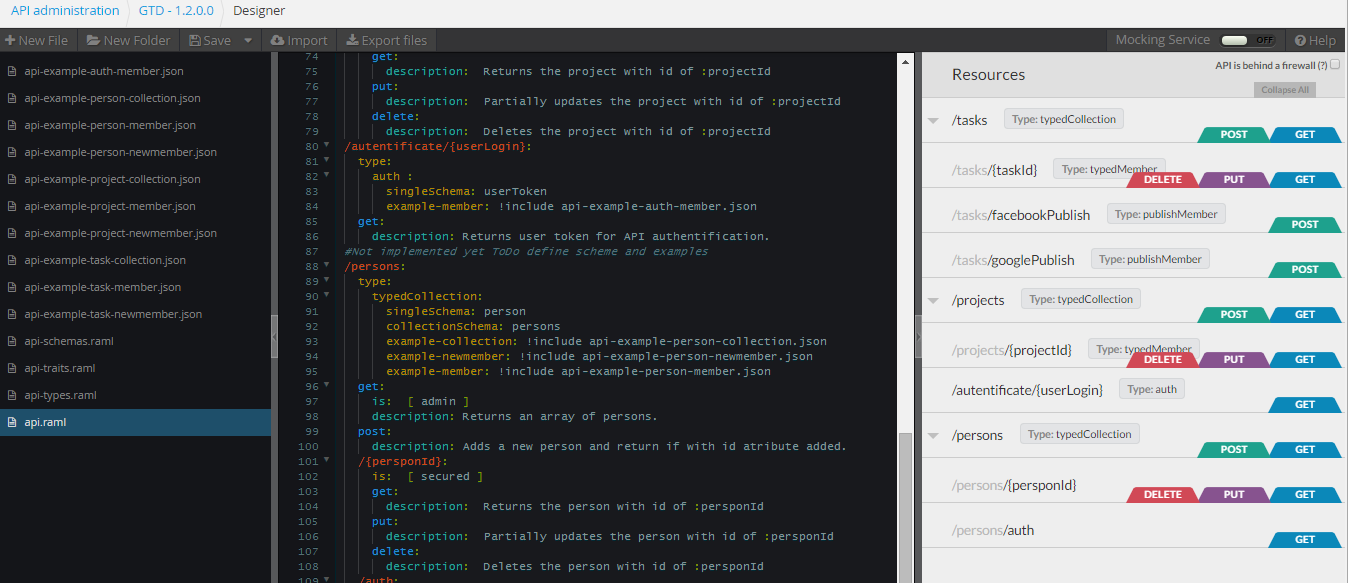
\includegraphics[width=1\textwidth]{pictures/gtd_raml_anypoint}
	\caption{Webové prostředí pro návrh REST API ve specifikaci RAML od firmy Mulesoft}\label{fig:gtd_raml_ide}
\end{figure}

Práce s tímto prostředím je příjemná. Některé funkce potřebují ještě vylepšit. Chybí online nápověda v kontextu specifikace RAML a např. auto complete nepracuje s objekty vytvořenými uživatelem. Zároveň příkladů návrhu API v jazyku RAML na webu není mnoho. To bohužel prodlužuje čas učení a samotného návrhu. Přesto má tento nástroj vykročeno stát se součástí moderního vývoje \cite{ws_raml_ddd}. 

\section{Databázový model}
\label{design:database_model}
V \ref{technology:hibernate} jsem se rozhodli pro použití Hibernatu. To nám umožňuje specifikovat strukturu databáze přímo v datovém modelu aplikace. Specifikace se provádí pomocí anotací nad objekty tříd, metod a atributů\cite{design_hibernate_annotations}. 

\chapter{Realizace}
\todo{verze knihoven}
V této kapitole se seznámíme s praktickým použitím dříve zvolených technologií. U aplikace pro centrální uložení dat si ukážeme strukturu projektu, podobu práce s REST API, generování struktury databáze pomocí frameworku hibernat, identifikace uživatele s použitím tokenu a práci s API Facebooku či Google kalendáře.
U android aplikace si uk\todo{co s ukážeme u android aplikace}
\newpage

\todo{blbe sekce}

\section{Aplikace pro centrální uložení dat}

Zde si ukážeme části implementace aplikace pro centrální uložení dat.

\subsection{Struktura projektu}
 
\begin{figure}[h!]
\dirtree{%
.1 libs\DTcomment{externí knihovny používané aplikací}.
.1 src\DTcomment{základní balík implementace projektu}.
.2 main\DTcomment{balík aplikace}.
.3 java\DTcomment{složka s kódy aplikace}.
.4 GTD\DTcomment{základní balík GTD}.
.5 BL\DTcomment{balík business vrstvy}.
.5 DL\DTcomment{balík datové vrstvy}.
.5 restapi\DTcomment{balík pro REST API}.
.3 resources\DTcomment{složka obsahující konfigurace}.
.4 database\DTcomment{složka obsahující pomocné skripty pro správu databáze}.
.4 messages\DTcomment{složka pro stringové konstanty aplikace}.
.4 gtd.api.properties\DTcomment{property aplikace}.
.4 hibernate.cfg.xml\DTcomment{konfigurace hibernatu}.
.4 logback.xml\DTcomment{konfigurace logování pomocí logbacku}.
.2 test\DTcomment{složka obsahující unit testy}.
.1 build.gradle\DTcomment{build soubor pro Gradle}.
.1 settings.gradle\DTcomment{nastavení Gradlu}.
}
\end{figure}

\subsection{Spring MVC}

\textit{Implementace je rozdělena na několika úrovní:}
\begin{itemize}[nosep]
	\item \textit{kontrolery}
	\item \textit{servisy}  
	\item \textit{persistence dat}	
\end{itemize}

\textit{Kontrolery}

Jejich úkolem je přijetí požadavku a odeslání odpovědi. Samotné zpracování delegují na servisy. Příklad v \ref{realization:restapi_controller}.

\lstinputlisting[label=realization:restapi_controller,caption=Příklad třídy kontroleru]{codes/controller_task.java}

\textit{Servisy}

Na této úrovni se odehrává business logika. Každá servisa obsluhuje funkce pro zpracování konkrétní entity (např. task/projekt). Využívá k tomu vlastní implementaci, další servisy a datovou vrstvu příslušnou entitě kterou obsluhuje. Příklad v \ref{realization:restapi_servise}.

\lstinputlisting[label=realization:restapi_servise,caption=Příklad třídy servisy]{codes/servise_person.java}

\textit{Persistence dat}

Využívá Hibernatu \ref{technology:hibernate} s implementací generiky\cite{realization_hibernate_generic} pro základní operace. Příklad v 

\lstinputlisting[label=realization:restapi_controller,caption=Příklad třídy kontroleru]{codes/dao_person.java}

\subsection{Databáze}

Příklad použití anotací na základě \ref{realization:hibernate_example}.

\lstinputlisting[label=realization:hibernate_example,caption=Příklad použití Hiberante]{codes/hibernate_person.java}

Význam anotací dle \cite{design_hibernate_annotations}.

Doplněním anotací k prvkům datového modelu a konfigurací hibernatu byla v MySQL vygenerována následující databázová struktura \ref{fig:gtd_database_model}.

\begin{figure}
	\makebox[\textwidth][c]{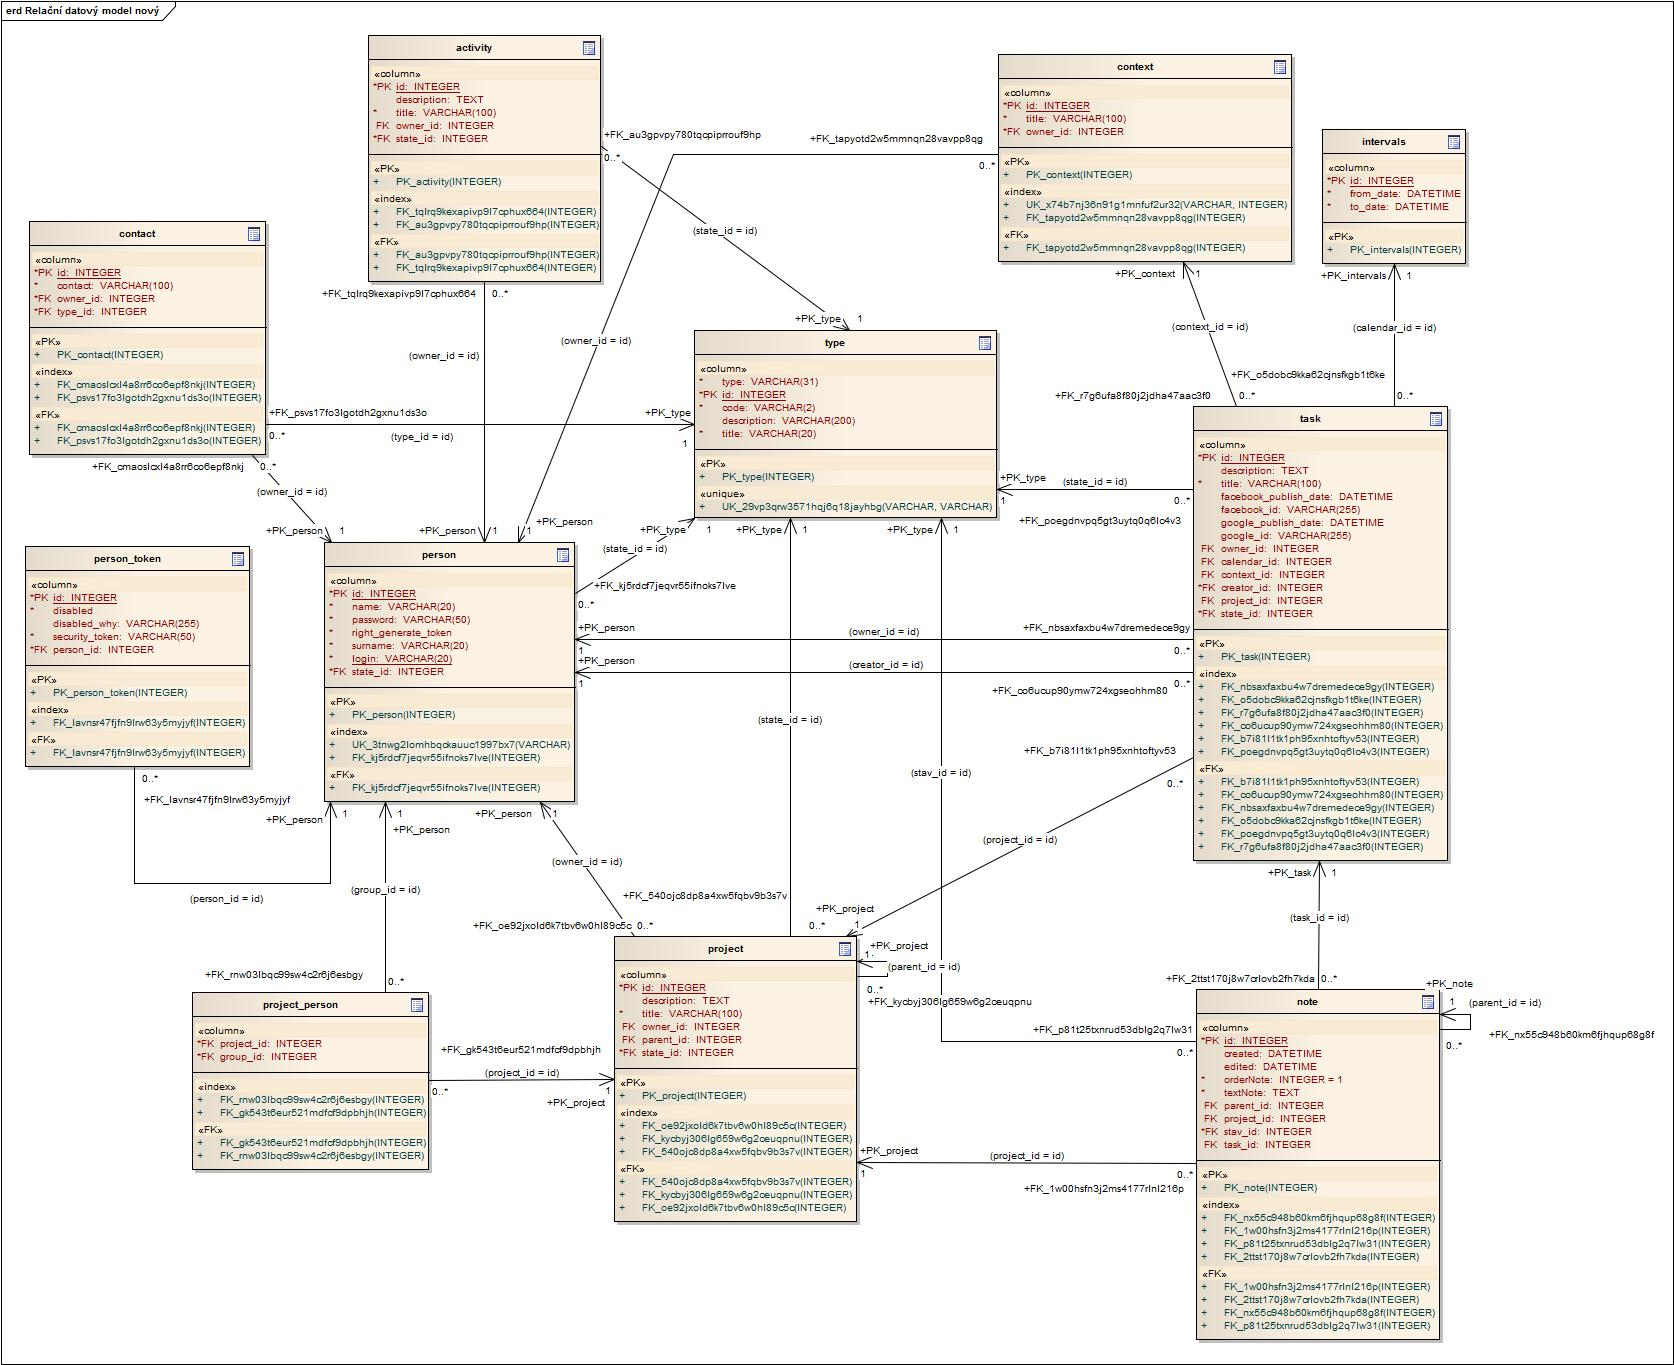
\includegraphics[height=1.17\textwidth, angle=90]{pictures/gtd_entity_relationship_diagram}}
	\caption{Databázový model}\label{fig:gtd_database_model}
\end{figure}

\subsection{Identifikace uživatele}
\label{realization:user_autentorization}
Identifikace uživatele je realizována formou tokenu v hlavičce HTTP požadavku. Token lze získat pomocí dvou způsobů (viz. \ref{tab:RESTfulAPI_rozhrani_bez}):
\begin{itemize}[nosep]
	\item \textit{registrací} -- po vytvoření účtu je ve vráceném objektu \textit{osoby} obsažen také token
	\item \textit{přihlášení} -- autentifikace pomocí loginu a hesla uživatele, v takovém případě je zpět vrácen pouze token a login uživatele.
\end{itemize}

Při vytvoření uživatele je token vygenerován automaticky. V případě přihlášení je vrácen aktivní token uživatele. Pokud uživatel token nemá (např. token byl deaktivován) a má právo si token vytvořit, je mu automaticky vygenerován.

Pokud uživatel už aktivní token má, může použít dotaz číslo 17 z \ref{tab:RESTfulAPI_rozhrani_s}. API na základě tokenu rozpozná \textit{osobu} a vrátí její objekt \textit{osoby} obsahující všechny tokeny. 

Token je generován pomocí kódu v \ref{api_token_generated} (person je objekt typu Person).

\begin{lstlisting}[label=api_token_generated,caption=Generování uživatelského tokenu]
	String stringToCrypt = person.toString() + PersonToken.tokenSalt + currentTimeMillis();
	String hash = HashConverter.md5(stringToCrypt);
\end{lstlisting}

Samotná kontrola tokenu v příchozím požadavku je realizována pomocí implementace vlastního filtru\cite{realization_spring_filter} viz. \ref{realization:auth_token_check}. 

\lstinputlisting[label=realization:auth_token_check,caption=Filter pro kontrolu tokenu]{codes/auth_token_check.java}

\subsection{Facebook}
\label{realization:restapi_facebook}

\todo{Co je tu - obecn2 uvody do kapitol lepe}
Podoba adresy pro publikaci úkolu na Facebook je v tabulce \ref{tab:RESTfulAPI_rozhrani_s} pod číslem 11. Z adresy je určen úkol, který se má publikovat a v těle požadavku je zaslán access token\ref{design:facebook_divide_appliaction}. 

O publikování se stará třída FacebookPublisher využívající restfb\ref{design:technology_restfb}. Její ukázka \ref{realization:restapi_facebookpublisher}.
\vspace*{1\baselineskip}
\newline
Kroky ke zpracování požadavku:
\begin{enumerate}[nosep]
	\item \textit{přijetí požadavku}
	\item \textit{získání instancí uživatele a úkolu} 
	\item \textit{kontrola, jestli byl požadavek už dříve publikován} -- stejný úkol lze znovu odeslat po 24 hodinách od prvního odeslání	
	\item \textit{vytvoření instance třídy facebookPublisher} -- v konstruktoru je předán access token
	\item \textit{z úkolu je vytvořena textová zpráva} 
	\item \textit{publikace zprávy pomoci restfb} 
	\item \textit{kontrola vráceného id zprávy} -- po vytvoření Facebook API vrátí identifikaci vzniklého objektu
	\item \textit{aktualizace úkolu o datu publikace a id zprávy}
	\item \textit{konec zpracování}
\end{enumerate}

\lstinputlisting[label=realization:restapi_facebookpublisher,caption=Ukázka ze třídy FacebookPublisher]{codes/facebook_publish.java}

\subsection{Google}

Řešení je podobné verzi s Facebookem \ref{realization:restapi_facebook}.

Implementace čerpá z ukázky na \cite{design_google_quickstart}. Využíváme Google knihoven. Ty umožňují autorizaci pomocí access tokenu a poskytují specializované rozhraní pro publikaci na API Google kalendáře.

O publikování se stará třída GooglePublisher. Její ukázka \ref{realization:restapi_googlepublisher}.
\vspace*{1\baselineskip}
\newline
Kroky ke zpracování požadavku:
\begin{enumerate}[nosep]
	\item \textit{přijetí požadavku}
	\item \textit{získání instancí uživatele a úkolu} 
	\item \textit{kontrola, jestli úkol nebyl dříve publikován a jedná se o úkol ve stavu v kalendáři}
	\item \textit{vytvoření instance třídy googlePublisher} -- v konstruktoru je předán access token
	\item \textit{vytvořena instance event z dat úkolu} 
	\item \textit{publikace zprávy pomoci google api} 
	\item \textit{kontrola vráceného id eventu} -- po vytvoření Googlee API vrátí identifikaci vzniklého objektu
	\item \textit{aktualizace úkolu o datu publikace a id eventu}
	\item \textit{konec zpracování}
\end{enumerate}

\lstinputlisting[label=realization:restapi_googlepublisher,caption=Ukázka ze třídy GooglePublisher]{codes/google_publish.java}



\section{Mobilní aplikace pro Android}

Dále si ukážeme části implementace aplikace pro centrální uložení dat.

\subsection{Struktura projektu}

Projekt respektuje konvenci pro adresářovou strukturu \cite{realization_androi_project_structure}.

\begin{figure}[h!]
	\dirtree{%
		.1 libs\DTcomment{externí knihovny používané aplikací}.
		.1 src\DTcomment{základní balík implementace projektu}.
		.2 main\DTcomment{balík aplikace}.
		.3 assets\DTcomment{soubory k použití}.
		.3 java\DTcomment{složka s kódy aplikace}.
		.4 cz.slama.android.gtd\DTcomment{balík GTD}.
		.3 res\DTcomment{resoursy aplikace}.
		.3 AndroidManifest.xml\DTcomment{manifest pro android aplikaci}.
		.1 build.gradle\DTcomment{build soubor pro Gradle}.
		.1 default.properties\DTcomment{property aplikace}.
	}
\end{figure}

Za zmínku stojí soubor AndroidManifest.xml. Android systém ho používá jako zdroj základních informací o aplikaci\cite{realization_androi_manifest}. 

\subsection{Klient pro konzumaci REST API}

\todo{blbe reference}
Retrofit \ref{technology:android_client_for_restapi} je potřeba nejdříve nakonfigurovat viz \ref{retrofit_configuration}. V naší konfiguraci definujeme základní část URL, interceptor pro přidání tokenu\ref{realization:user_autentorization} do HTTP hlavičky,
\begin{itemize}[nosep]
	\item \textit{společná část URL pro všechny požadavky} \ref{rest_api_design} 
	\item \textit{errorhandler} -- zavolá se při chybě požadavku (chyba spojení, chybový HTTP status \cite{http_statuses}, \dots)
	\item \textit{interceptor pro přidání tokenu} \ref{realization:user_autentorization}
	\item \textit{úroveň logování}
	\item \textit{parser pro data} -- data jsou ve formátu JSON a pro parsování je použita knihovna GSON \cite{retrofit_gson}.
\end{itemize}

\lstinputlisting[label=realization:retrofit_configuration,caption=Konfigurace Retrofit]{codes/retrofit_configuration.java}

Dalším krokem je specifikace rozhraní\footnote{https://docs.oracle.com/javase/tutorial/java/concepts/interface.html} pro volání konkrétního API (příklad je v \ref{realization:retrofit_interface}). Rozhraní definuje adresu volaného API (k hodnotě je přidána společná URL) a parametry vstupu/ výstupu.

\lstinputlisting[label=realization:retrofit_interface,caption=Definice rozhraní pro Retrofit]{codes/retrofit_interface.java}

A konečně propojíme předešlé dva body \ref{realization:retrofit_boostrap}. Příklad volání \ref{retrofit_example_call}.

\lstinputlisting[label=realization:retrofit_boostrap,caption=Třída pro práci s Retrofit]{codes/retrofit_bootstrap_service.java}

\lstinputlisting[label=retrofit_example_call,caption=Příklad volání Retrofit]{codes/retrofit_example.java}

\subsection{Asynchronní načítání dat}

Práce s daty přes REST API je operace vyžadující čas. Takovou operaci nesmíme provádět v hlavním vlákně aplikace\cite{android_threads}. Protože spuštění náročné operace v hlavním vlákně vede z pohledu uživatele k \uv{zamrznutí} aplikace. Co hůře, pokud je vlákno vytíženo déle jak 5 s dojde k zobrazení hlášení \uv{application not responding}. Řešením je asynchronní zpracování, které neblokuje hlavní vlákno, ale vytváří si vlastní.

Implementace asynchronního zpracování je součástí \ref{technologie:androdi:boostrap}. Objekt se jmenuje \textit{SafeAsyncTask}.

Příklad takového zpracování \ref{adnroid_async_task}. Funkce \textit{handleAction} je volána při stisku tlačítka pro akci u úkolu. 
\begin{itemize}[nosep]
	\item \textit{uživatel klikl na tlačítko pro akci u úkolu} -- pro řešení této události je u tlačítka registrována funkce \textit{handleAction} 
	\item \textit{zkontrolujeme, že asynchronní task neexistuje} -- ochrana, abychom task nespustili vícekrát
	\item \textit{vytvoříme task typu SafeAsyncTask} -- překryjeme funkce podle zamýšleného chování
	\item \textit{task spustíme}
\end{itemize}

Za zmínku stojí dvě cesty pro zpracování výjimek. Jedna je součástí samotného asynchronní části \textit{onException}. V případě chyby při volání API \ref{Klient pro konzumaci REST API} jsou volány zaregistrování posluchači pro konkrétní události. Požita je knihovna Otto\cite{android_otto}. V ukázce jsou posluchači funkce s anotací \textit{@Subscribe}.

\lstinputlisting[label=adnroid_async_task,caption=Příklad asynchronního volání]{codes/android_asyncTasks.java}

\subsection{Facebook}
\label{realization:android_facebook}

Podle postupu v \ref{technology:facebook_sdk} byla aplikace zaregistrována na Facebook\ref{fig:facebok_registration}. Kromě názvu balíku a hlavní aktivity\cite{android_launcher_activity} je pro registraci potřeba získat hash klíče, kterým je aplikace podepsána\cite{android_signing}. Vzor pro získání hashe je v \ref{facebook_key_hash}. 

\begin{lstlisting}[label=facebook_key_hash,caption=Získání hashe vývojového klíče Android prostředí]
keytool -exportcert -alias androiddebugkey -keystore %HOMEPATH%\.android\debug.keystore | openssl sha1 -binary | openssl base64
\end{lstlisting}
  
\begin{figure}[h!]\centering
	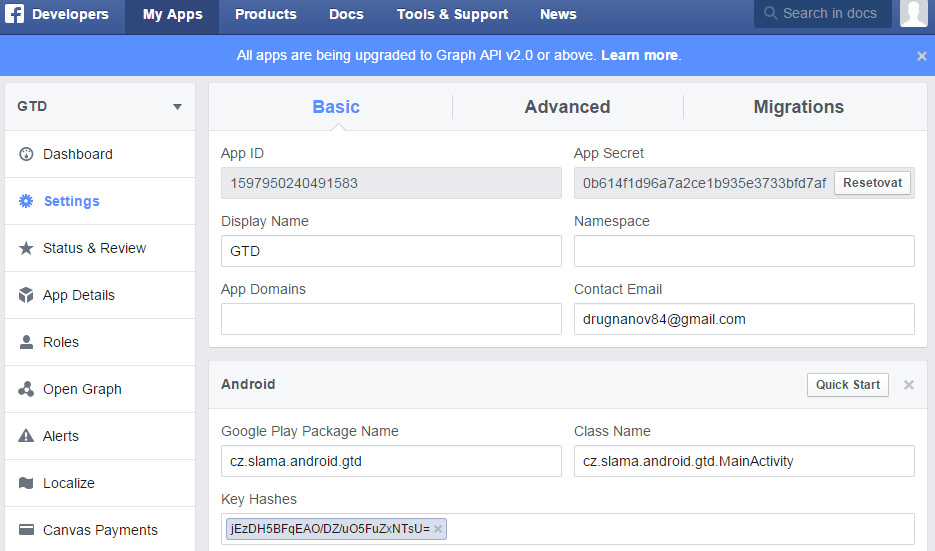
\includegraphics[width=1\textwidth]{pictures/facebook_app_registration.png}
	\caption{Registrace aplikace na Facebook}
	\label{fig:facebok_registration}
\end{figure}

Po registraci je aplikaci přiděleno \textit{App id} a \textit{App secret}. Ty potřebujeme v následující konfiguraci podle \cite{android_facebook_manifest}. Příklad našeho manifestu \ref{adnroid_facebook_manifest}.

\lstinputlisting[label=adnroid_facebook_manifest,caption=Konfigurace Facebooku v manifestu Android aplikace]{codes/facebook_manifest.xml}

Facebook SDK je třeba před použitím inicializovat\ref{facebook_sdk_init}.
\begin{lstlisting}[label=facebook_sdk_init,caption=Inicializace Facebook SDK]
FacebookSdk.sdkInitialize(getApplicationContext())
\end{lstlisting}

Komponenta tlačítka od Facebooku, které spravuje přihlášení/ odhlášení uživatele, je \textit{com.facebook.login.widget.LoginButton}.\newline

Zbývajícím krokem je implementace pro získání access tokenu \ref{facebook_login}. Postup je následující. 
\begin{itemize}[nosep]
	\item \textit{specifikujeme požadovaná práva} -- pomocí \textit{setPublishPermissions} nastavíme požadovaná oprávnění, která budou uživateli předložena ke schválení 
	\item \textit{registrujeme callbacky}
	\item \textit{získání access tokenu} -- po úspěšném přihlášení dostáváme objekt typu LoginResult a z něj access token. Úspěšný login ale nemusí znamenat přidělení všech práv, o která jsme žádali. Proto kontrolujeme, jestli nedošlo k jejich zamítnutí.
	\item \textit{uložení access tokenu} -- access token ukládáme do tzv. shared preferences\cite{android_shared_prefereces}.
\end{itemize}

\lstinputlisting[label=facebook_login,caption=Získání access tokenu s použitím Facebook SDK]{codes/facebook_login.java}

\subsection{Google}
\label{realization:android_google}

Postup přihlášení a získání access tokenu je podobný tomu u Facebooku\ref{realization:android_facebook}. Dále si popíšeme důležité odlišnosti. 

Budeme postupovat podle návodu \cite{android_google_guide}.

Výsledkem registrace naší aplikace na google konzoli je \ref{fig:google_registration}. Pro získání fingerprintu byl použit postup uvedený na \cite{android_google_fingerprint}.

\todo{co to je za obrazek?}
\begin{figure}[h!]\centering
	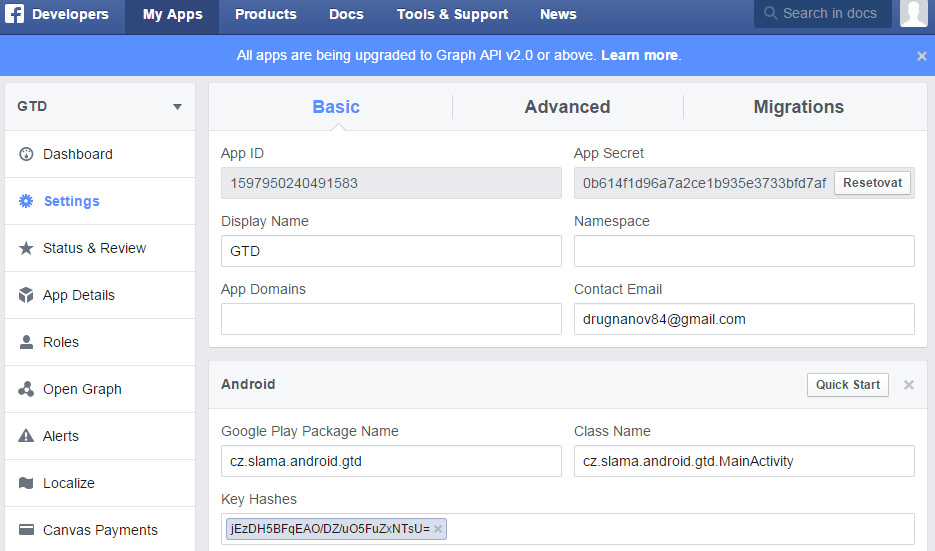
\includegraphics[width=1\textwidth]{pictures/facebook_app_registration.png}
	\caption{Registrace aplikace na Google}
	\label{fig:google_registration}
\end{figure}

Do manifestu potřebujeme zanést verzi použitých Google play services\cite{google_manifest_version} a práva aplikace pro správu účtů \ref{google_manifest_rights}.

\begin{lstlisting}[label=realization:google_manifest_version,caption=Konfigurace Android manifestu pro Google play services]
<meta-data android:name="com.google.android.gms.version" android:value="@integer/google_play_services_version"/>
\end{lstlisting}

\begin{lstlisting}[label=realization:google_manifest_rights,caption=Konfigurace Android manifestu pro získání práv ke správě účtů]
<uses-permission android:name="android.permission.GET_ACCOUNTS"/>
<uses-permission android:name="android.permission.MANAGE_ACCOUNTS"/>
<uses-permission android:name="android.permission.AUTHENTICATE_ACCOUNTS"/>
<uses-permission android:name="android.permission.USE_CREDENTIALS"/>
\end{lstlisting}

Stejně jako Facebooku budeme pro správu přihlášení používat komponentu od Googlu \textit{com.google.android.gms.common.SignInButton}.\newline

Kroky pro získání access tokenu podle \ref{facebook_login} jsou následující.
\begin{itemize}[nosep]
	\item \textit{přihlášení uživatele k jeho google účtu} -- zajišťuje komponenta \textit{com.google.android.gms.common.SignInButton}.
	\item \textit{specifikujeme požadovaná práva} -- v předešlém bodě nemůžeme ještě žádat o rozšířená práva pro naši aplikaci\cite{android_google_incremental_scopes}. Práva si připravíme (proměnná \textit{SCOPE\_TO\_USE}) a v dalším bodě o ně zažádáme.
	\item \textit{žádost o rozšířená práva} -- uživatel je přihlášen ke svému google účtu a máme připravená práva pro aplikace. Přes třídu \textit{GoogleAuthUtil} o ně požádáme. Uživateli je zobrazeno dialogové okno s žádostí o jejich potvrzení.
	\item \textit{získání access tokenu} -- výstupem předešlého bodu je access token, který ukládáme do shared preferences\cite{android_shared_prefereces}.
\end{itemize}

\lstinputlisting[label=facebook_login,caption=Získání access tokenu přes Google play services]{codes/google_login.java} 

\section{DigitalOcean - instalace}

V \ref{technology:hosting} jsme pro hostování zvolil server DigitalOcean.
\newline
Nastavení hostingu je v tabulce \ref{tab:digitalocean_configure}.

\begin{table}[h!]\centering
	\caption{Současné nastavení hostingu na serveru DigitalOcean tokenu}\label{tab:digitalocean_configure}
	\begin{tabular}{l l}
		Operační systém:&Ubuntu 14.04\footnote{www.ubuntu.com}\\
		Databáze:&MySQL verze 5.5.41\footnote{www.mysql.com}\\
		Admin databáze:&phpMyAdmin verze 4.0.10deb1\footnote{http://www.phpmyadmin.net}  \\	
		Aplikační server:&WildFly verze 8.2.0.Final\footnote{http://wildfly.org/}\\	
	\end{tabular}
\end{table}

Nyní si projdeme postup pro jeho instalaci.
\begin{enumerate}[nosep]
	\item \textit{vytvoření dropletu} -- nejdříve je třeba vytvořit droplet. Postupujeme podle návodu \cite{digitalocean_droplet}. Současně získáme přihlašovací údaje pro vzdálené připojení.
	\item \textit{vzdálené připojení náš server} -- využijeme např.mobaxterm\footnote{mobaxterm.mobatek.net} 
	\item \textit{instalace Javy} -- návod na \cite{digitalocean_java} 
	\item \textit{instalace WildFly} -- návod na \cite{digitalocean_wildfly}
	\item \textit{instalace MySQL} -- návod na \cite{digitalocean_wildfly}
	\item \textit{instalace phpMyAdmin} -- návod na \cite{digitalocean_phpMyAdmin} 
\end{enumerate}

\section{GitHub}

Pro zálohování zdrojových kódu a samotné bakalářské práce je použit Git Hub.\newline 

Repozitáře jsou na Git Hubu umístěny na adrese \textit{github.com/Drugnanov}.

Návod pro používání např. \cite{github_guide}.

\chapter{Testování aplikace}

Pro testování REST API vznikl SOAP UI\cite{testing_soapui} projekt (viz. \ref{fig:soapui}). Obsahuje seznam požadavků zasílaných na REST API. Parametry požadavku jako token nebo content-type jsou součástí nastavení zdrojů pro celou URL a podřízené požadavky je automaticky dědí. 

\begin{figure}[h!]\centering
	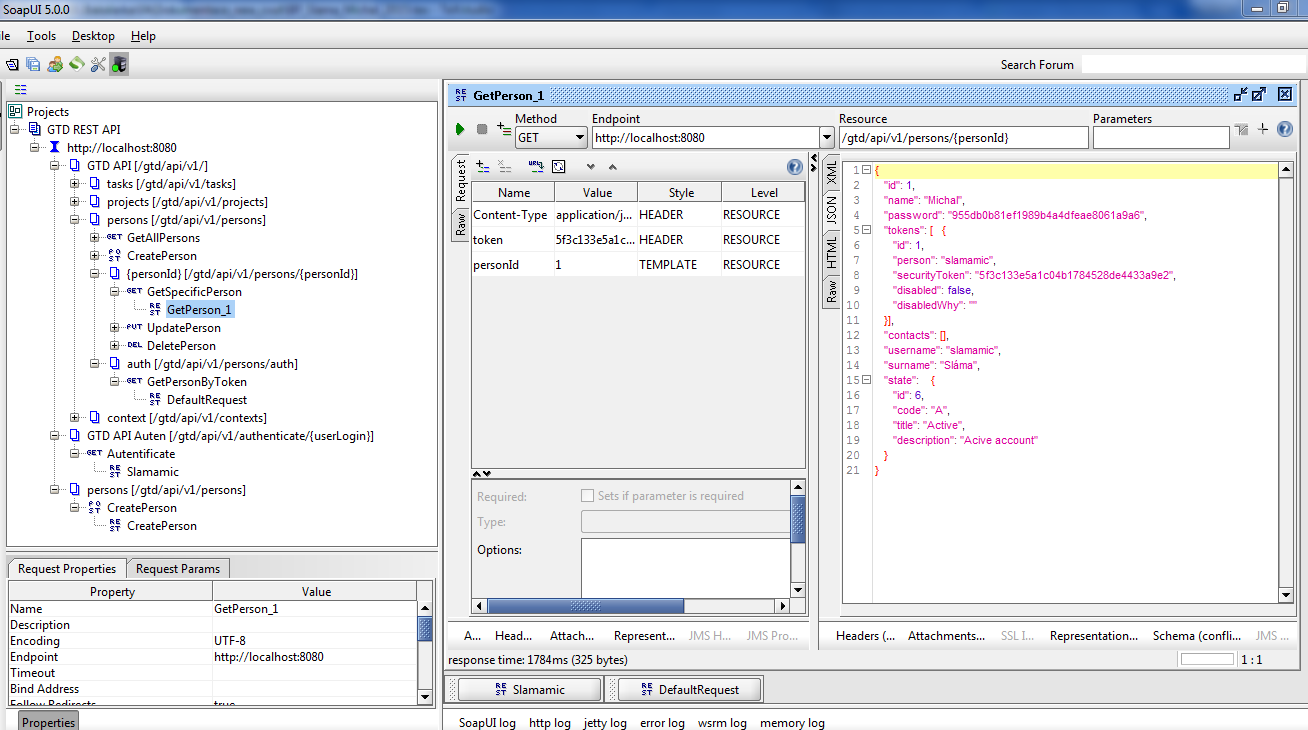
\includegraphics[width=1\textwidth]{pictures/sopaui}
	\caption{Projekt SOAP UI pro testování RESP API}
	\label{fig:soapui}
\end{figure}


\chapter{Návrhy k rozvoji}

\todo{více propojit}
Zde uvádím další návrh pro rozvoj aplikace. Návrhy jsou seřazeny od neprioritnějšího.\newline

Přejít do fáze testování s uživateli. Ověřit chování a fungování na reálných zařízeních. Získat zpětnou vazbu od uživatelů. Tu vyhodnotit a navrhnout další úpravy funkcí a vzhledu.  

Využít HTML 5 \cite{todo_html5} a s pomocí existujících frameworků (např. Sencha \cite{todo_sencha}) vytvořit aplikaci podporující více platforem. 

Napojení na emailové schránky. Téměř každý člověk, který přijde do styku s internetem disponuje také emailovým účtem \cite{todo_email_stats}. Současně právě přijetí nebo napsání emailu vytváří pro uživatele úkol. Proto dalším rozvojem je napojení na emailové servery (např. Gmail\footnote{mail.google.com}, MS Outlook\footnote{www.microsoft.com/cs-cz/outlook-com/}, \dots). Kteří to budou a co vše by takové napojení mělo znamenat, bude součástí další analýzy. 

Opravit webovou aplikaci vzniklou v rámci předmětu SP2. Ta přestala fungovat na základě změn v aplikaci centrálního uložení dat souvisejících s touto bakalářskou prací.

\begin{conclusion}

Metodika \GTD do mého života přinesla nový směr a podle něj se snažím řídit. Mysl potřebujeme použít k řešení problému a ne jako diář, který ještě funguje velmi podivně a události nám připomíná velmi nahodile. Diář si musíme vytvořit mimo ni. Na internetu nám k tomu pomůže celá řada produktů. Je jen na nás, který si vybereme. A volba je důležitá. Protože metodika nás nabádá, že musíme mít naprostou důvěru ke spolehlivosti svého systému a používat ho rádi. Plánování a revize úkolů se musí stát pravidelnou činností, ke které se nemusíme přemlouvat.

Z pohledu systému metodika definuje základní objekty typu projekt a úkol, jejich stavy a postup zpracování. Jedná se jednoduchý proces, přičemž u systému je kladen důraz na jednoduchost ovládání a spolehlivost. 

Existující řešení disponují širokým záběrem podporovaných platforem a přehledným ovládáním. Hlavní slabinu vidím v převážně chybějící podpoře pro integraci s dalšími programy (emaily, sociální sítě, \dots).

Proto můj návrh neobsahuje speciální funkce pro osobní plánování, ale předpokládá integraci na Facebook a Google kalendář.

Aplikace pro centrální uložení dat je v současnosti nasazena na hostingu serveru DigitalOcean. Díky zvolené kombinaci technologií Spring/ Hibernate/ REST API byl její vývoj bez výrazných komplikací.

Aplikace pro OS Android je nasazena a testována na lokálním emulátoru. Testování probíhá ve spolupráci s mou rodinnou, kdy sbírám podměty k dalším úpravám. V blízké době dojde k nasazení na reálná zařízení a rozšíření testovacích uživatelů. První verzi aplikace vystavěnou na prázdném projetu jsem pro nepřehlednost kódu zahodil a s využitím Android Bootstrap \ref{technologie:androdi:boostrap} projektu postavil novou. Byl to důsledek, že se jedná o mou první Android aplikace a s tím je spojení učení za pochodu.      

Integrace s Facebook a Google kalendářem je implementována a funguje. Uživatel může v Android aplikaci použít přihlášení ke svému Facebook/ Google účtů a publikovat vlastní úkol na zeď Facebooku nebo do kalendáře Googlu. Naplnil jsem navrhl k oddělené funkce publikování na dvě části a to získání přístupových práv a samotné publikování. To představuje zjednodušení pro další vývoj uživatelských aplikací.

Získaných zkušeností si velice cením. Instalace a správa hostingu, REST API, technologie a principy Android aplikace společně s nastavením vývojového prostředí, napojení na Facebook a Google, \dots. To jsou zkušenosti, které určitě využiji ve svém dalším profesním životě a další práci na tomto projektu.
 

%Framework Spring, který jsem použil pro aplikaci poskytující centrální uložení dat, mi pomohl k vytvoření dobře škálovatelné a udržovatelné aplikace. Vybrané REST API dostálo mým předpokladům, pro které jsem ho vybral. Implementace není náročná na straně serveru ani klienta a plně vyhovuje potřebám aplikace. Stejně tak má volba Hibernatu pro \acrshort{orm} řešení mě dobře odstínila od databázového prostředí. Zde se ukazuje síla anotací. Pomocí nich lze provádět širokou škálu konfigurací bez nutnosti externích konfiguračních souborů. Proto jsem pomocí anotací konfiguroval  samotnou aplikaci a zde mi práci ulehčil vybraný Spring Boot. 
%
%Pro hosting jsem zvolil server Digiocean. Zde jsem vytvořil vlastní Linux server, nainstaloval a nakonfiguroval aplikační server WildFly a databázi MySQL s phpAdminem a nasadil REST API aplikaci.
%
%Mobilní aplikaci jsem vyvinul a testoval na lokálním emulátoru Genymotion s instalovanou verzí Androidu 19. Volba Bootstrapu byla výborná a pro účely mé aplikace plně vyhovující. Framework poskytuje dostačující infrastrukturu a zároveň je sám založen na další knihovnách usnadňujících vývoj. 
%
%Nastudoval jsem specifikace API Facebooku a Google kalendáře. Umožňuji uživateli publikovat úkol na jeho vlastní zeď Facebooku. Stejně může publikovat úkol do Google kalendáře. Zde jsem správně navrhl oddělit funkci publikování na dvě části a to získání přístupových práv a samotné publikování. Přístupová práva získává Android aplikace a k tomu využívá komponenty přímo od Facebooku a Googlu. Správně jsem analyzoval, že proces nelze automatizovat, ale vytvořením přístupového tokenu lze následné publikování delegovat na jinou aplikaci. O samotné publikování se stará REST API aplikace.
%
%Práce s API Facebook i Googlu pro mě znamenala cennou zkušenost a vidím v něm velký potenciál dalšího rozvoje. V moderním internetovém prostředí už nemůže aplikace existovat izolovaně, ale je třeba ji integrovat do existujícího prostředí. A tato integrace nemá být pouze pasivní, ale také aktivní.
%
%....kolik lidí to použivá
\todo{na čem je nasazeno, kolik lidí to používá a další rozvoj}

\end{conclusion}

\bibliographystyle{csn690}
\bibliography{mybibliographyfile}

\appendix

\chapter{Seznam použitých zkratek}
\printglossaries


\chapter{Obsah přiloženého CD}

%upravte podle skutecnosti

\begin{figure}
	\dirtree{%
		.1 readme.txt\DTcomment{stručný popis obsahu CD}.
		.1 exe\DTcomment{adresář se spustitelnou formou implementace}.
		.1 src.
		.2 impl\DTcomment{zdrojové kódy implementace}.
		.2 thesis\DTcomment{zdrojová forma práce ve formátu \LaTeX{}}.
		.1 text\DTcomment{text práce}.
		.2 thesis.pdf\DTcomment{text práce ve formátu PDF}.
		.2 thesis.ps\DTcomment{text práce ve formátu PS}.
	}
\end{figure}

\end{document}
